\documentclass[a4paper,fleqn,usenatbib]{mnras}

%=========================================================================
\usepackage{amsmath} 
\usepackage{amssymb} 
\usepackage{graphicx}
\usepackage{grffile}
\usepackage[dvips]{epsfig}
\usepackage{epsfig}  
\usepackage{color}
\usepackage{caption}
\usepackage{hyperref}
\usepackage{bm}
%Non reposionated tables




%=========================================================================
%		INTERNAL MACROS
%=========================================================================
\def\be{\begin{equation}}
\def\ee{\end{equation}}
\def\ba{\begin{eqnarray}}
\def\ea{\end{eqnarray}}

% To highlight comments 
\definecolor{red}{rgb}{1,0.0,0.0}
\newcommand{\red}{\color{red}}
\definecolor{darkgreen}{rgb}{0.0,0.5,0.0}
\newcommand{\SRK}[1]{\textcolor{darkgreen}{\bf SRK: \textit{#1}}}
\newcommand{\SRKED}[1]{\textcolor{darkgreen}{\bf #1}}
\newcommand{\before}[1]{\textcolor{red}{ #1}}
\newcommand{\after}[1]{\textcolor{darkgreen}{ #1}}
\newcommand{\hs}{{\hspace{1mm}}}  
\newcommand{\tol}{Tololo 1214-277}
\newcommand{\HI}{{\text{H\MakeUppercase{\romannumeral 1}}} }
\newcommand{\HII}{{\text{H\MakeUppercase{\romannumeral 2}}} }
\newcommand{\lya}{\ifmmode{{\rm Ly}\alpha}\else Ly$\alpha$\ \fi}
\newcommand{\cm}{\ifmmode{{\rm cm}}\else cm\fi}
\newcommand{\ccm}{\,\mathrm{cm}^{-3}}
\newcommand{\ergps}{\,{\rm erg}\,{\rm s}\ifmmode{}^{-1}\else ${}^{-1}$\fi}
\newcommand{\Mpch}{\,{\rm Mpc}\,\ifmmode h^{-1}\else $h^{-1}$\fi}
\newcommand{\dd}{\mathrm{d}}
\newcommand{\vek}[1]{\bm{#1}}
\newcommand{\hb}{H$\beta$}
\newcommand{\ha}{H$\alpha$}
\newcommand{\oiii}{[OIII]}
\newcommand{\oii}{[OII]}
\newcommand{\nii}{[NII]}
\newcommand{\esca}{erg cm$^{-2}$ s$^{-1}$ \AA$^{-1}$}
\newcommand{\esc}{erg cm$^{-2}$ s$^{-1}$}
\newcommand{\es}{erg s$^{-1}$}
\newcommand{\esa}{erg s$^{-1}$}
\newcommand{\kms}{\ifmmode\mathrm{km\ s}^{-1}\else km s$^{-1}$\fi}
\newcommand{\hMsun}{{\ifmmode{h^{-1}{\rm{M_{\odot}}}}\else{$h^{-1}{\rm{M_{\odot}}}$}\fi}}
\newcommand{\Msun}{{\ifmmode{{\rm{M_{\odot}}}}\else{${\rm{M_{\odot}}}$}\fi}}

\newcommand{\jefr}[1]{\textcolor{darkgreen}{\bf JEFR: \textit{#1}}}

\begin{document}

%=========================================================================
%		FRONT MATTER
%=========================================================================
\title[Satellites in the MW and M31]{Joint Satellite Distributions in the Milky Way and Andromeda}
\author[J.E. Forero-Romero \& V. Arias]
{Jaime E. Forero-Romero $^{1}$ \thanks{je.forero@uniandes.edu.co},
Ver\'onica Arias$^1$\\
%%
$^1$ Departamento de F\'isica, Universidad de los Andes, Cra. 1
  No. 18A-10 Edificio Ip, CP 111711, Bogot\'a, Colombia \\
}

\maketitle

\begin{abstract}
We focus on the spatial distribution of bright ($M_V<-8$) satellites and
pairs of galaxies with similar masses, isolation and kinematic
configurations as the Local Group. 
\end{abstract}

\begin{keywords}Galaxies: halos --- Galaxies: high-redshift --- Galaxies: statistics
--- Dark Matter --- Methods: numerical 
\end{keywords}

\section{Introduction}

\section{Observational Characterists of Andromeda and the Milky Way}
\label{sec:obs}


\section{Local Group Analogues in the Illustris Simulation}
\label{sec:NumericalSetup}

We use publicly available data from the Illustris Project 
\citep{2014MNRAS.444.1518V}. 
This suite of cosmological simulations, performed using the quasi-Lagrangian
code AREPO \citep{2010MNRAS.401..791S}, follow the coupled evolution of dark 
matter and gas and includes parametrizations to account for the effects of
gas cooling, photoionization, star formation, stellar feedback, black
hole and super massive black hole feedback. 

The simulation volume is a cubic box of $75$ \Mpch\ on a side.
The cosmological parameters correspond to a $\Lambda$CDM cosmology
consistent with WMAP-9 measurements \citep{2013ApJS..208...19H}. 

We extract halo and galaxy information from the Illustris-1 simulation
which has the highest resolution in the current release of the
Illustris Project.
Illustris-1 has $1820^3$ dark matter particles and $1820^3$ initial gas
volumen elements. 
This corresponds to a dark matter particle mass of
$6.3\times 10^6$\Msun\ and a minimum mass for the baryonic volume
element of $8.0\times 10^7$\Msun. 
The corresponding spatial resolution is $1.4$ kpc for the dark matter
gravitational softening and $0.7$ kpc for the typical size of the
smallest gas cell size. 

 

\subsection{Sample Selection: Local Group Analogues}

We build a sample of Local Group Analgues (LGA) by performing a selection on
the stellar mass and isolation properties of the galaxies in the
simulation. The conditions to select LGA galaxies are the following.

\begin{itemize}
\item LGA galaxy pairs are composed by galaxies with stellar mass in the
range $1\times10^{10}\Msun <M_{\star}<1.5 \times 10^{11} \Msun$.
\item For each galaxy $A$ we find its closest galaxy $B$, if galaxy $A$ is also
the closest to halo $B$, the two halos are considered as a pair. 
Another way to phrase this selection is that pairs do not have
neighbors closer than the pair's separation.
\item The distance between the galaxies' center of
  mass must be in the range $500$ kpc $<d_{AB}<$ $1500$ kpc. 
\item For each galaxy in the pair there cannot be a galaxy more
  massive than the lightest galaxy in the pair within a radius of $2$
  Mpc. 
\item Each galaxy in the pair must have at least $5$ satellites
  brighter than  $M_V<-9$.
\end{itemize}

We find $11$ pairs with these conditions.
Figure \ref{fig:general} shows the stellar masses, maximum circular
velocities and the number of bright satellites for all the pairs in
the sample.

\begin{figure*}
\centering
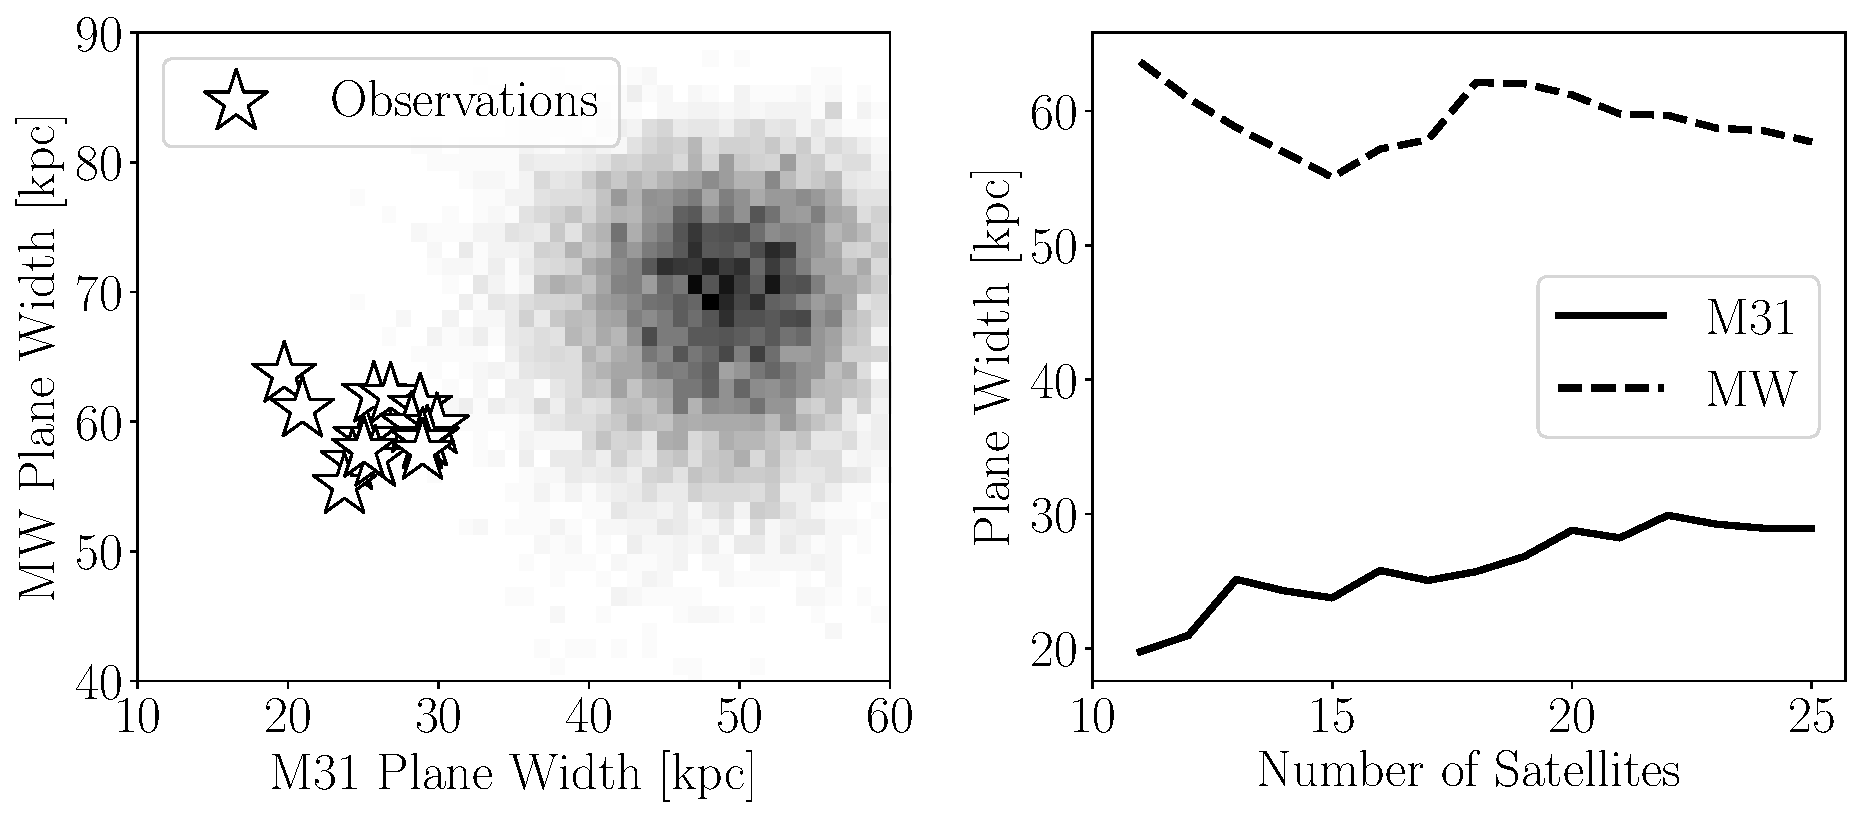
\includegraphics[width=0.7\textwidth]{planewidth_lg.pdf}
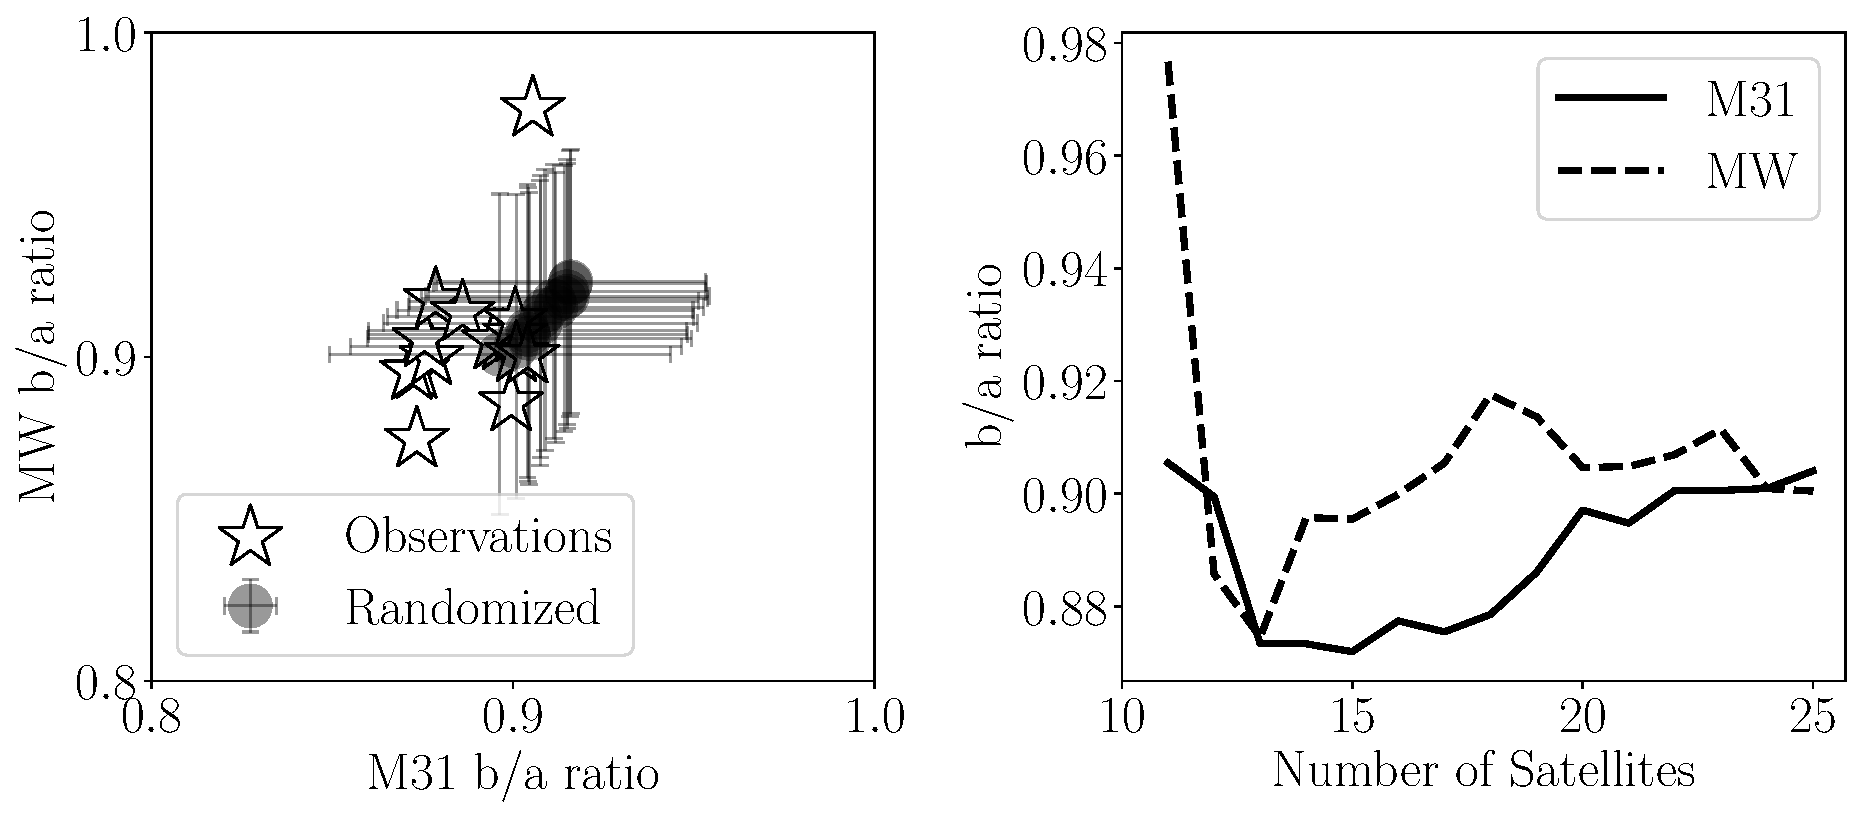
\includegraphics[width=0.7\textwidth]{ba_ratio_lg.pdf}
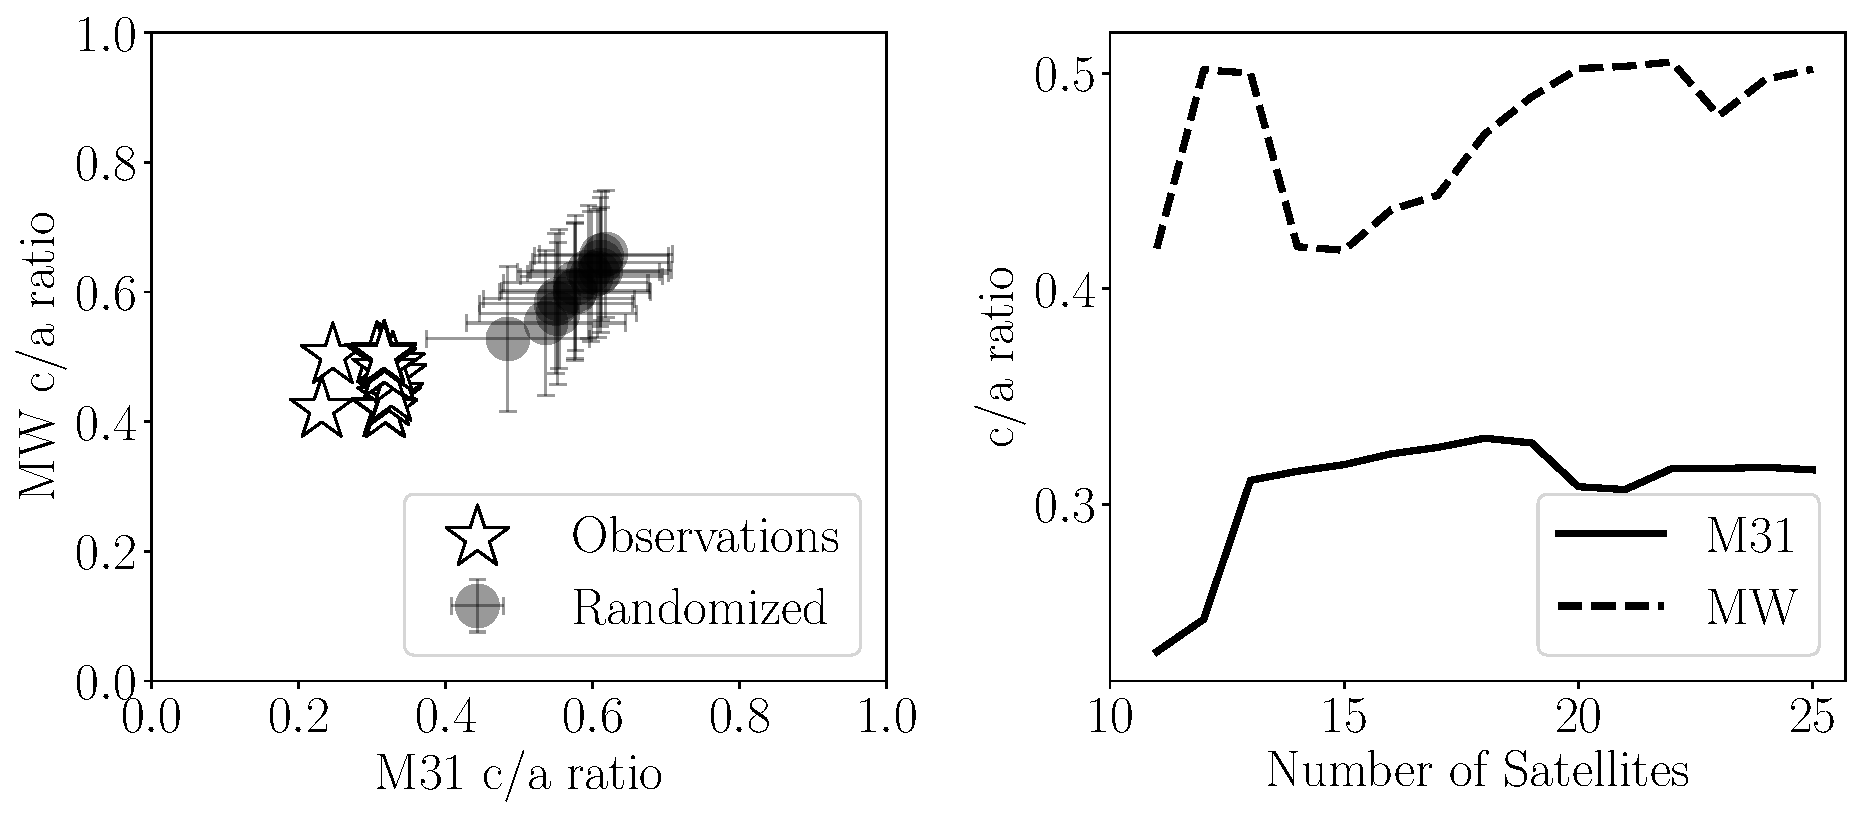
\includegraphics[width=0.7\textwidth]{ca_ratio_lg.pdf}
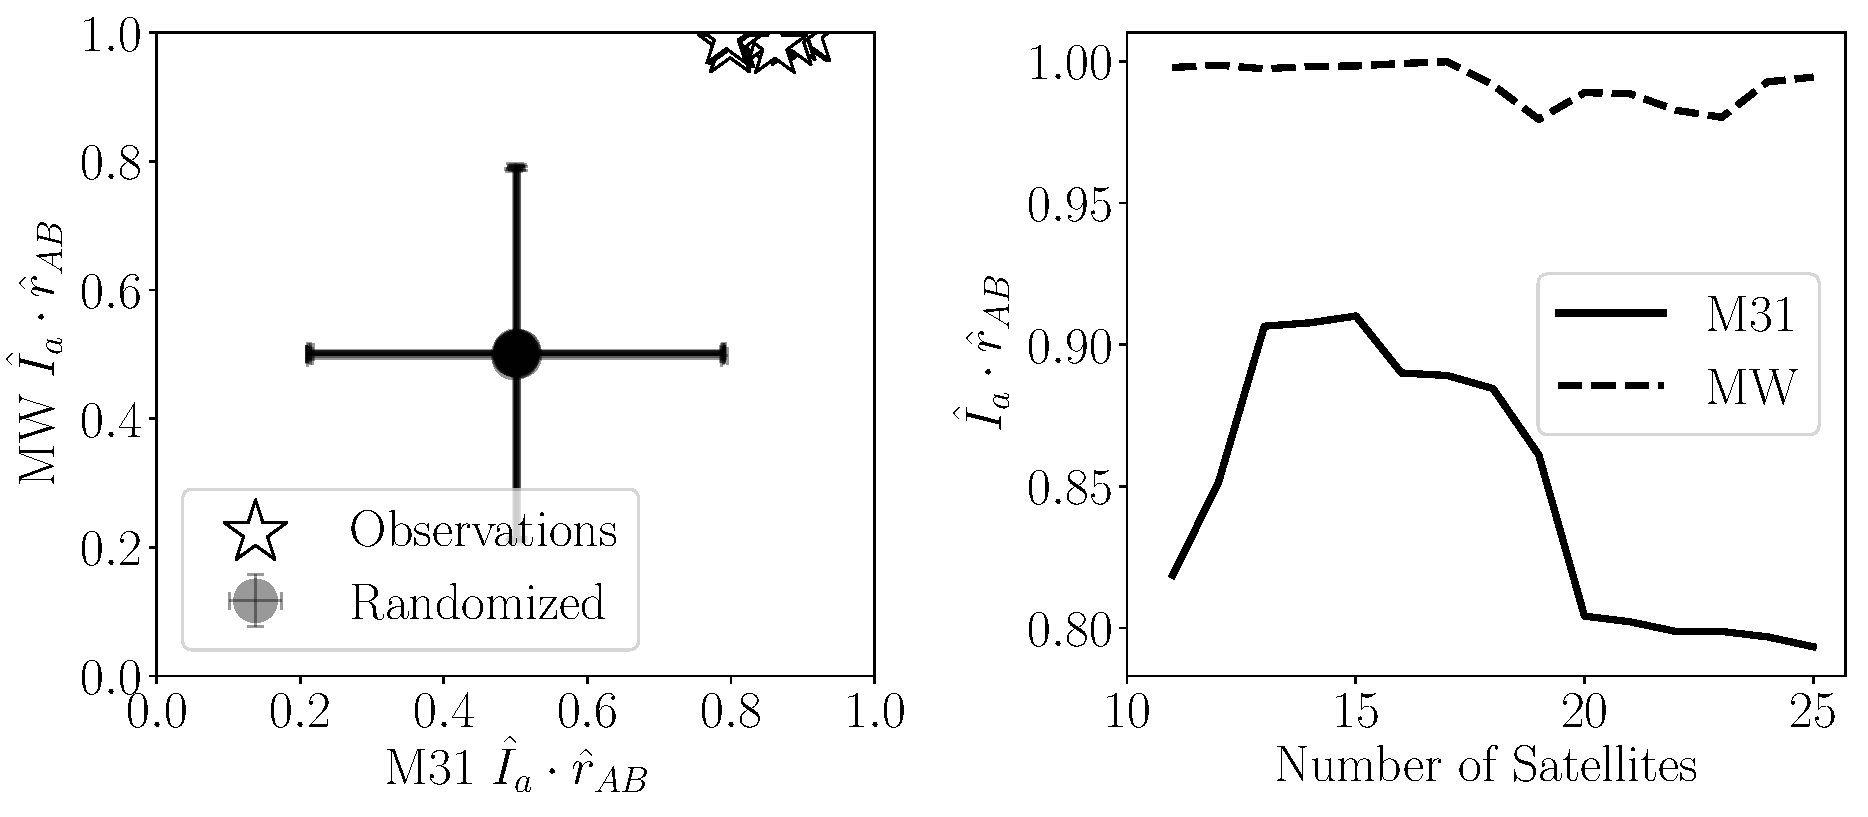
\includegraphics[width=0.7\textwidth]{mu_lg.pdf}
\caption{Basic characteristics for the MW and M31 satellite systems
\label{fig:general}}
\end{figure*}




\section{Satellite Spatial Distribution and Alignment}
\label{sec:SpatialMeasurements}

We characterize the bright ($M_V<-9$) satellite spatial distribution
with four different metrics. 

\begin{enumerate}
\item{The inertia tensor}.
\item{Fitting planes}.
\item{Velocity Anisotropy}.
\end{enumerate}

I what follows we describe the details of implementation of each
metric.


\subsection{Inertia Tensor}
\label{sub:inertia}
First, by computing the inertia tensor defined as 

\begin{equation}
{\bf{\bar{I}}} = \sum_{k \in V}[(\bf{r}_i - \bf{r}_0)^2\cdot \bf{1} -
  (\bf{r}_i-\bf{r}_0)\cdot (\bf{r}_i - \bf{r}_0)^{T}],
\end{equation}
%
where $k$ indexes the set of satellites of interest
$\bf{r}_k$ are the satellites' positions, $\bf{r}_{0}$ is the
positions pof the host DM halo, $\bf{1}$ is the unit matrix,  and
${\bf r}^T$ is the transposed vector $\bf{r}$. 
We finally compute the eigenvalues, $a>b>c$, and corresponding
eigenvectors, $\hat{I}_a$, $\hat{I}_b$, $\hat{I}_c$, of this tensor.
In the case of a sheet-like configuration the vector perpendicular to
the sheet would be signaled by, $\hat{I}_a$, the eigenvector of the
largest eigenvalue. 

% referencia posiciones satellites
% http://adsabs.harvard.edu/abs/2013MNRAS.435.1928P

\subsection{Plane fitting}
\label{sub:planes}

We fit satellite planes around each galaxy in the pair by randomly
generating 10000 unit vectors homogeneously distributed over the
sphere.
Each vector represents the direction perpendicular to a plane passing through
the main galaxy's center of mass. 
We compute the dot product of this unit vector with the position vector
for each satellite, this gives us the satellite distances to the
plane. 
The best plane is determined by the vector that gives the lowest
sample standard deviation in the satellite distances to the plane.
In the set of unit vectors to be considered we also include the vector
$\hat{I}_a$, which provides the exact solution in the case of $3$
satallites. 
We take the sample standard deviation as a measure of the plane's width
and denote by $\hat{p}$ the unit vector defining the direction
perpendicular to the best plane.
We also store the median of the satellite distances to the plane as a
measure of the plane's location with respect to the central galaxy.

\subsection{Velocity Anisotropy}
\label{sub:beta}

The velocity anisotropy paramenter, $\beta$ is defined as

\begin{equation}
  \beta = 1 - \frac{\sum_i v^2_{\rm{tan}; i}}{2\sum_i v^{2}_{\rm{rad};i}},
\label{eq:beta}
\end{equation}
% 
where $v_{\rm{tan/rad};i}$ correspond to the tangential/radial
velocity of the $i$-th satellite with respect to the central galaxy.



\begin{table*}
  \centering
\begin{tabular}{lll}
\hline\hline
Symbol & Units & Description\\\hline
$M_{\star}$ & $10^{10}$\Msun & Stellar mass of the central galaxy\\
$N_s$ & & Number of satellites with $M_V<-9$\\
$a > b> c$ & & Inertia tensor eigenvalues. \\
$\hat{I}_a$, $\hat{I}_b$, $\hat{I}_c$ & & Inertia tensor eigenvectors. \\
$\beta$  &  & Satellite Velocity Anisotropy\\
$\sigma_s$ & kpc & Plane width\\
$\hat{r}_{AB}$& & Unit vector in the direction to the galaxy companion\\
\hline\hline
\end{tabular}
  \caption{Overview of the parameters computed for each central galaxy
    and its satellite system.
  \label{tab:models}}
\end{table*}


\section{Results}
\label{sec:results}


\bibliographystyle{mnras}
\bibliography{Dwarfs}

%% Alignments between galaxies, satellite systems and haloes
%% https://arxiv.org/pdf/1605.01728.pdf

%% The tangential velocity excess of the Milky Way satellites
%% https://arxiv.org/pdf/1612.01529.pdf

%% Tambien deberiamos sacar las alineaciones con el momentum angular
%% de las estrellas de las galaxias principales.

%% http://adsabs.harvard.edu/abs/2017MNRAS.464.3825P

%M31 mass
%% https://arxiv.org/abs/1410.0017

%MW mass
%https://arxiv.org/abs/1407.1078


\end{document}

